\section{Diagrammes UML de Connect Four}


\begin{figure}[H]
    \centering
    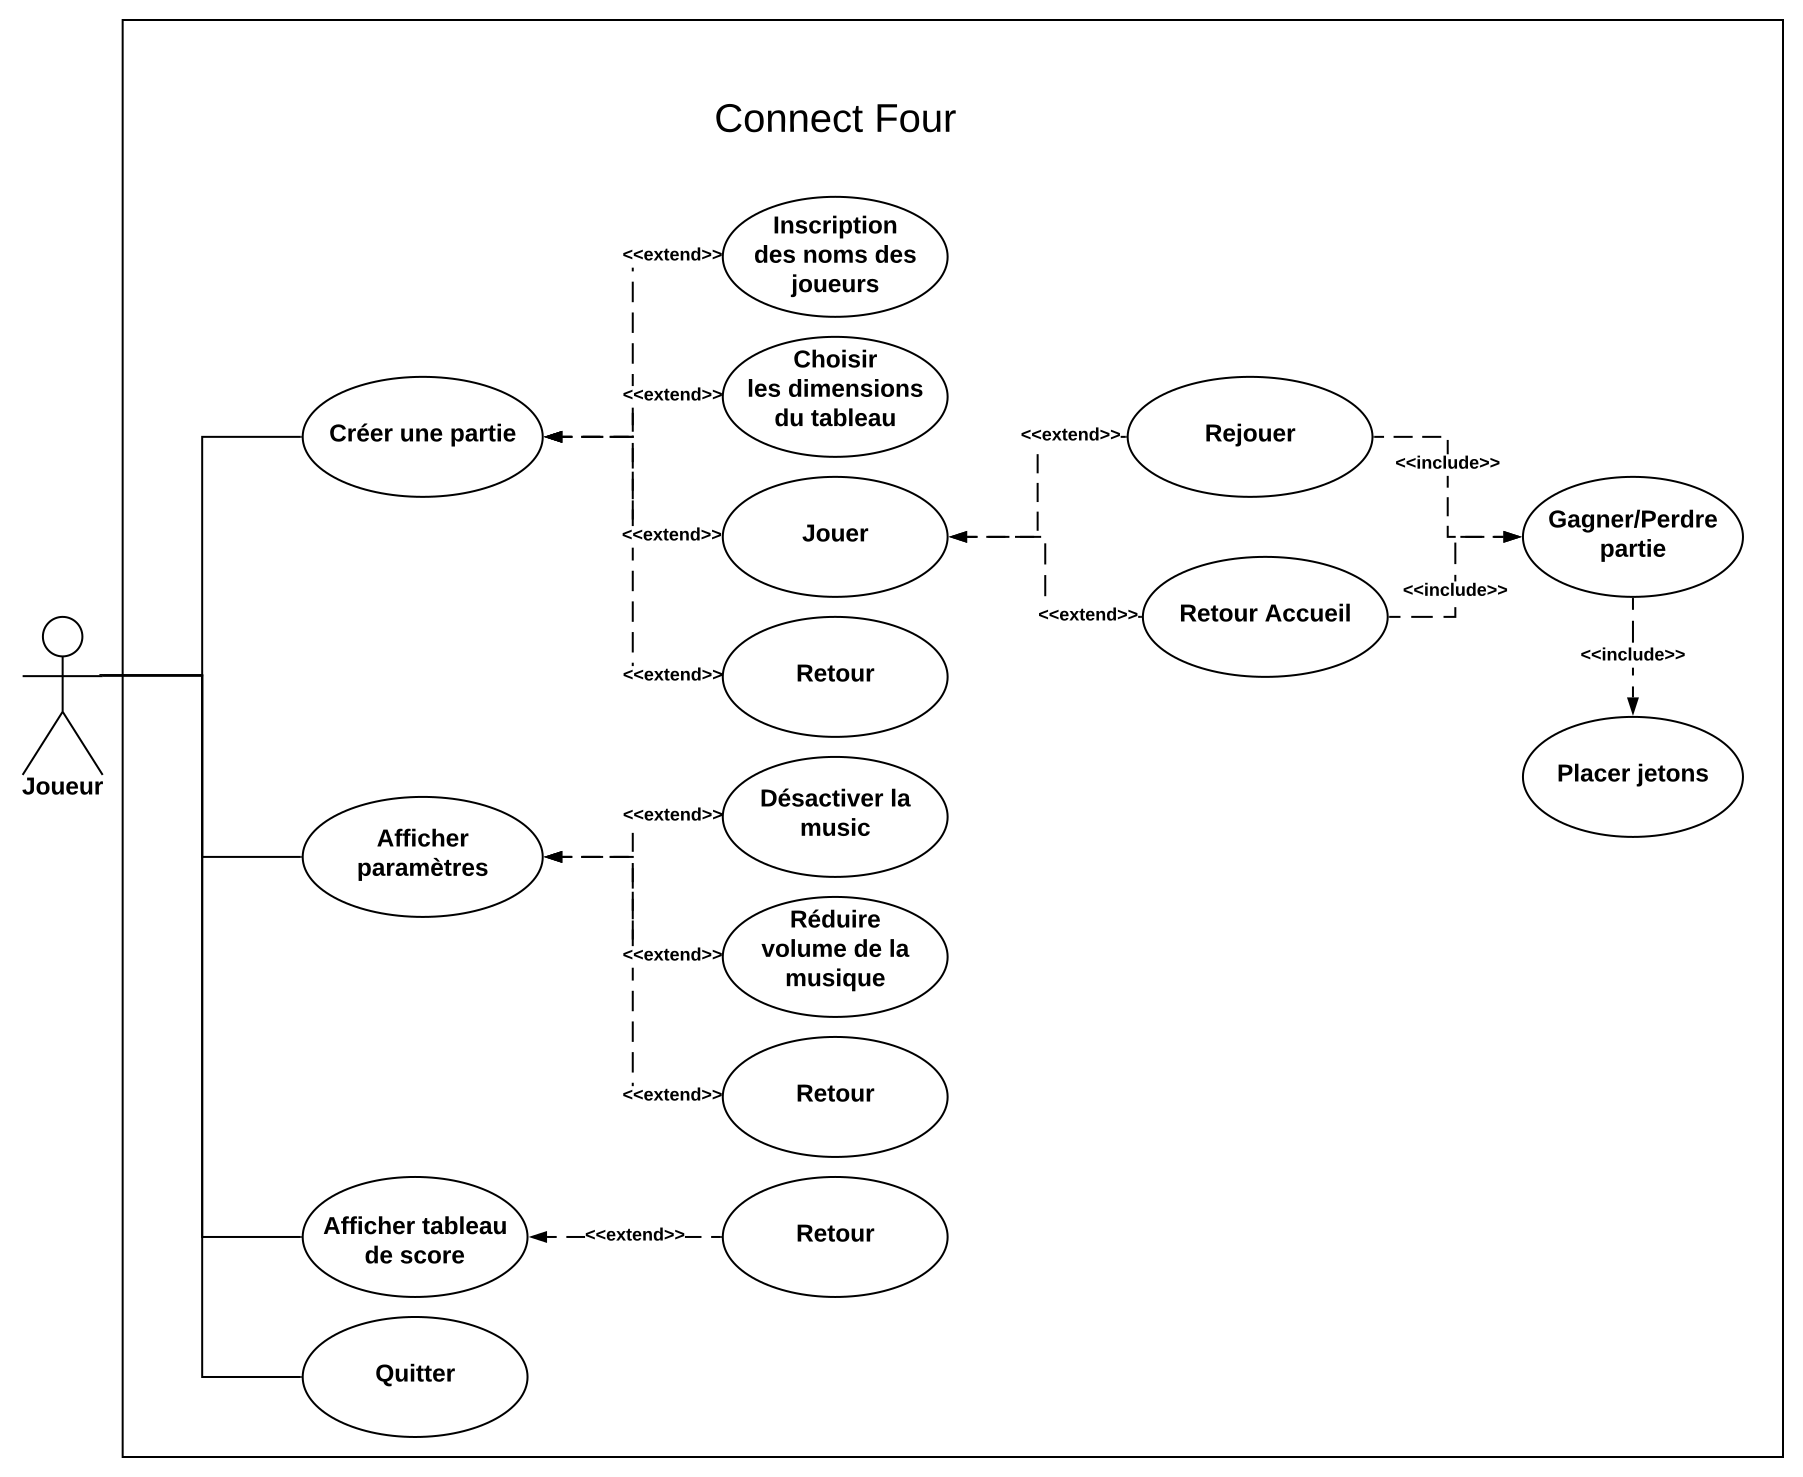
\includegraphics[width=6in]{img/cas}
    \caption{Diagramme de cas d’utilisation UML de haut niveau de Connect Four}
\end{figure}

\begin{figure}[H]
    \centering
    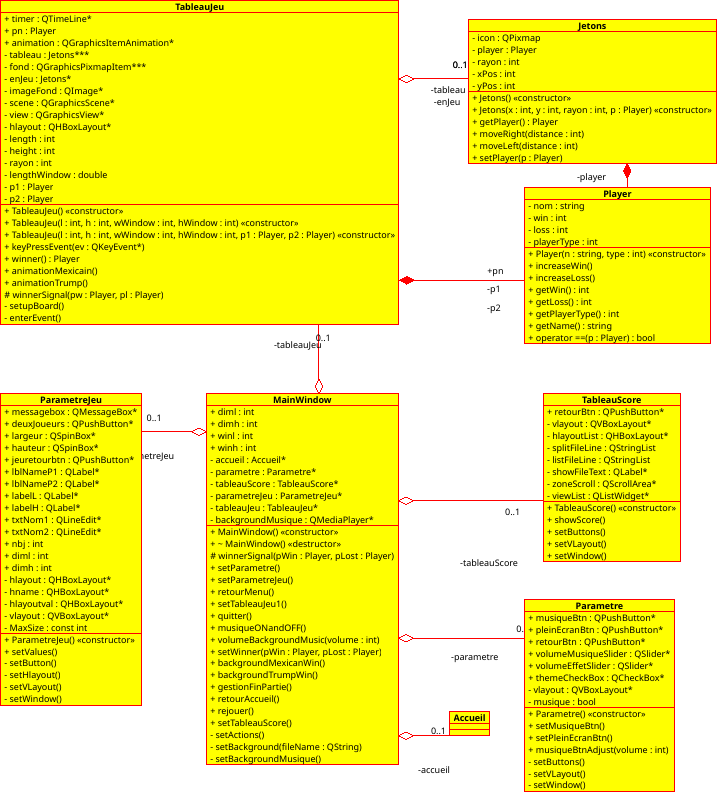
\includegraphics[width=6in]{img/classes}
    \caption{Diagramme de classe de Connect Four}
\end{figure}

\section{Captures d’écrans}

\begin{figure}[H]
    \centering
    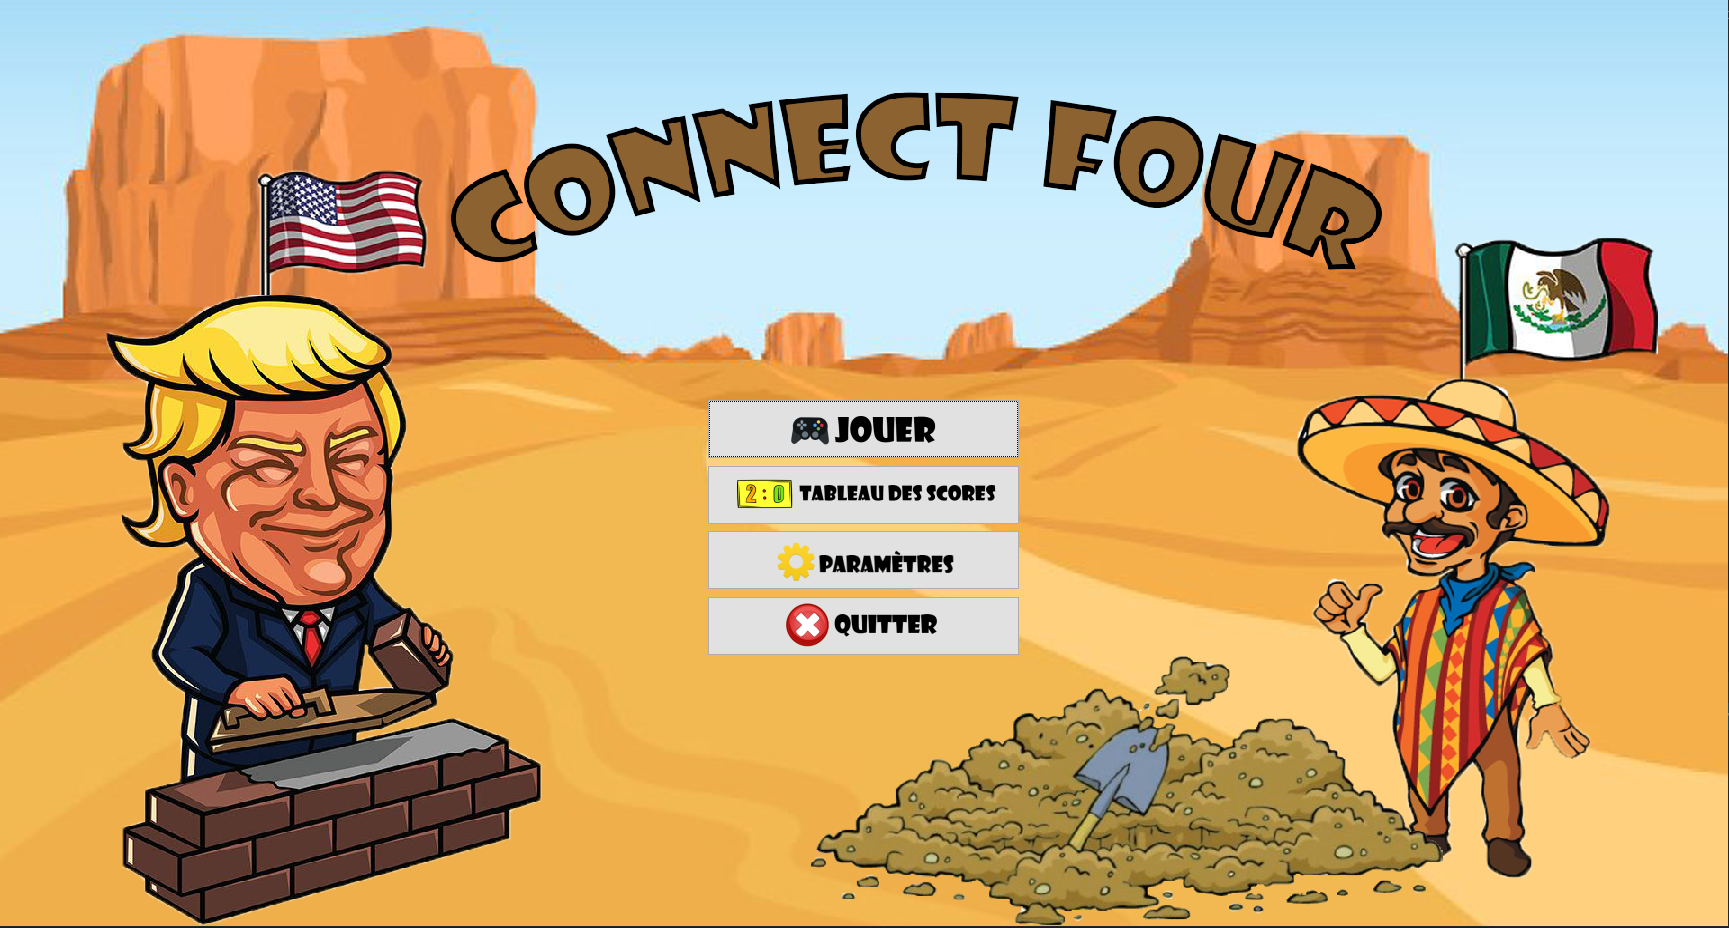
\includegraphics[width=6in]{img/1-accueil}
    \caption{Écran d'accueil}
\end{figure}

\begin{figure}[H]
    \centering
    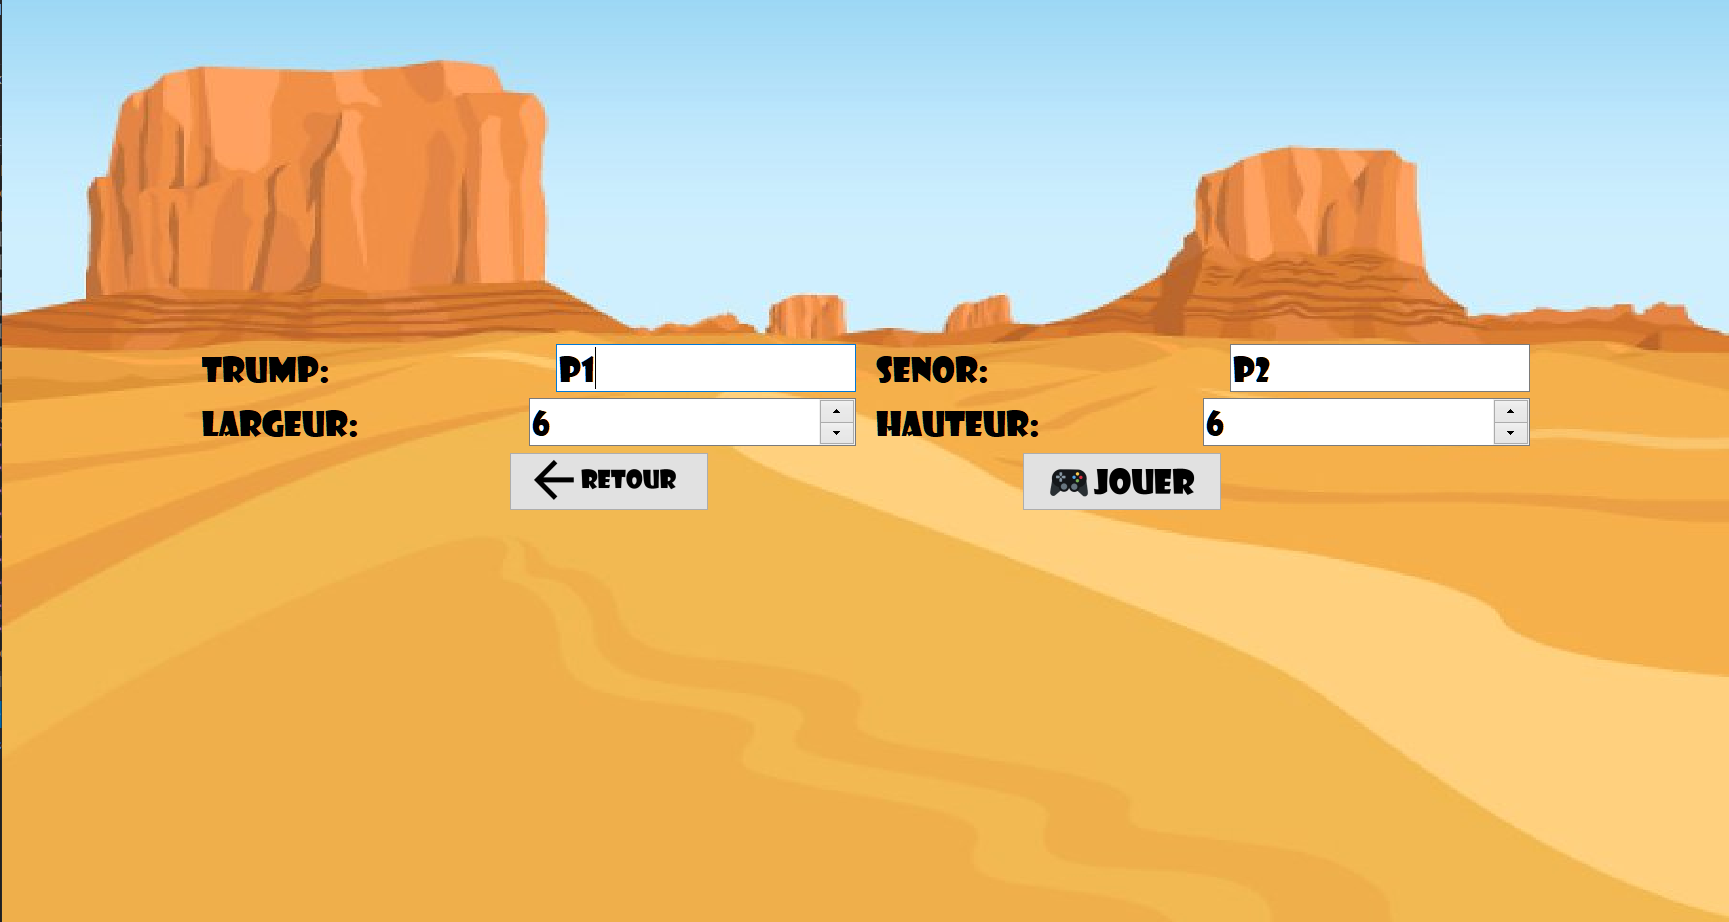
\includegraphics[width=6in]{img/2-parametreJeu}
    \caption{Écran des paramères du jeu}
\end{figure}

\begin{figure}[H]
    \centering
    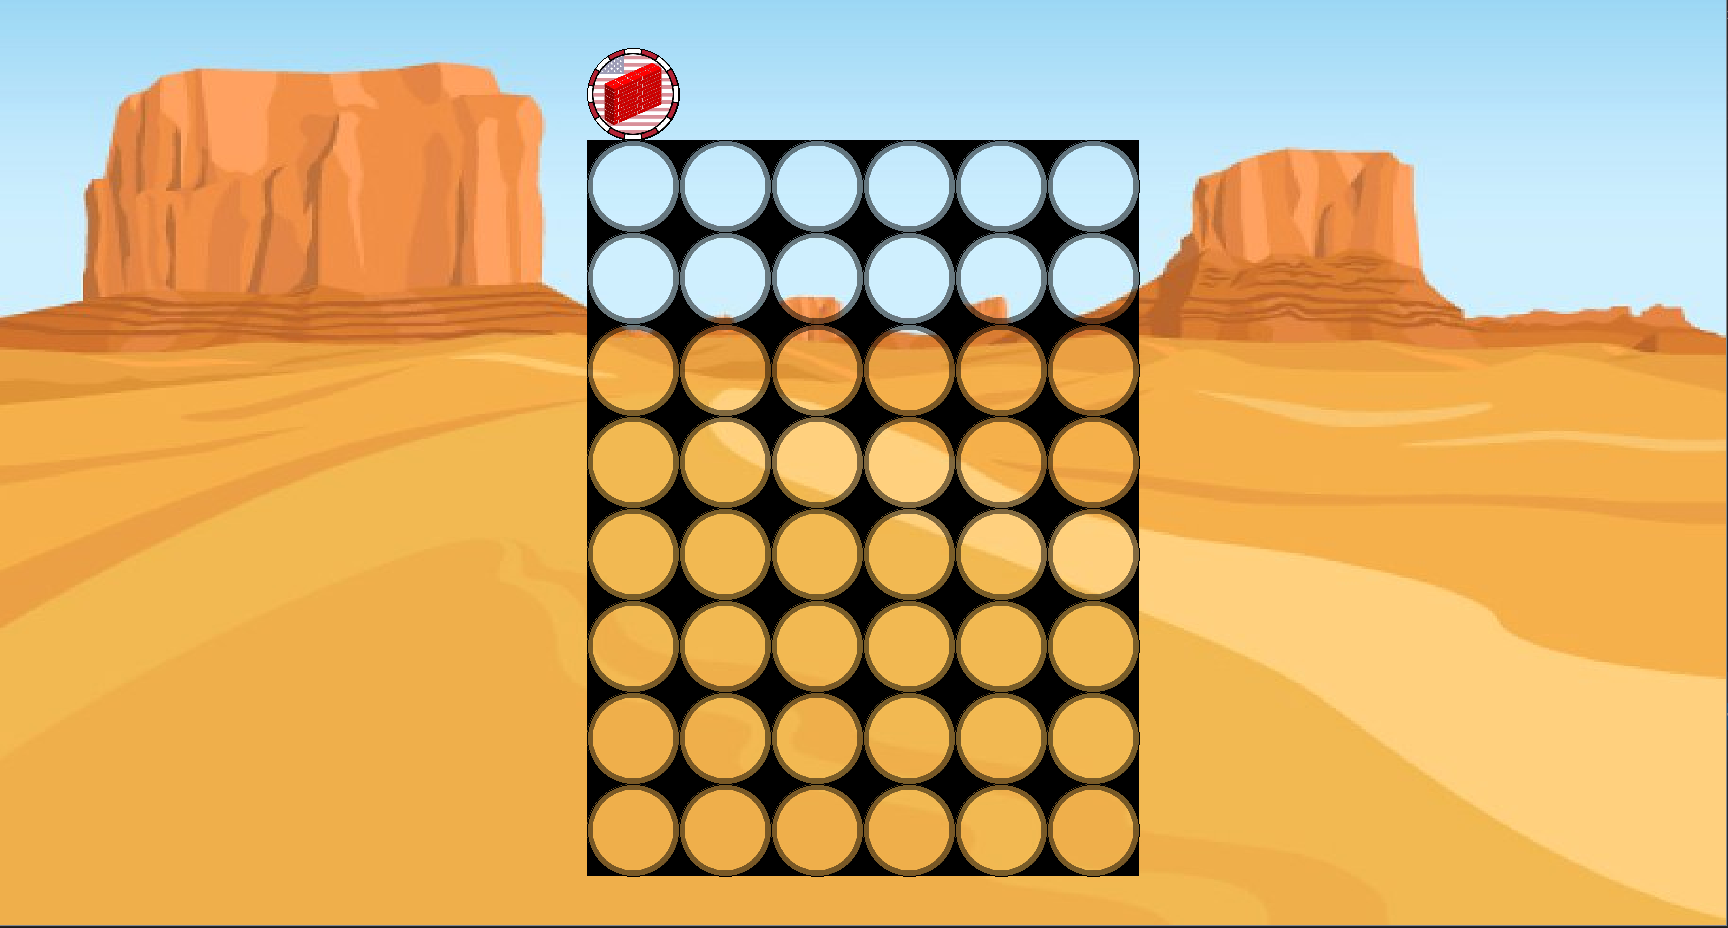
\includegraphics[width=6in]{img/3-tableauJeu}
    \caption{Écran du tableau de jeu}
\end{figure}

\begin{figure}[H]
    \centering
    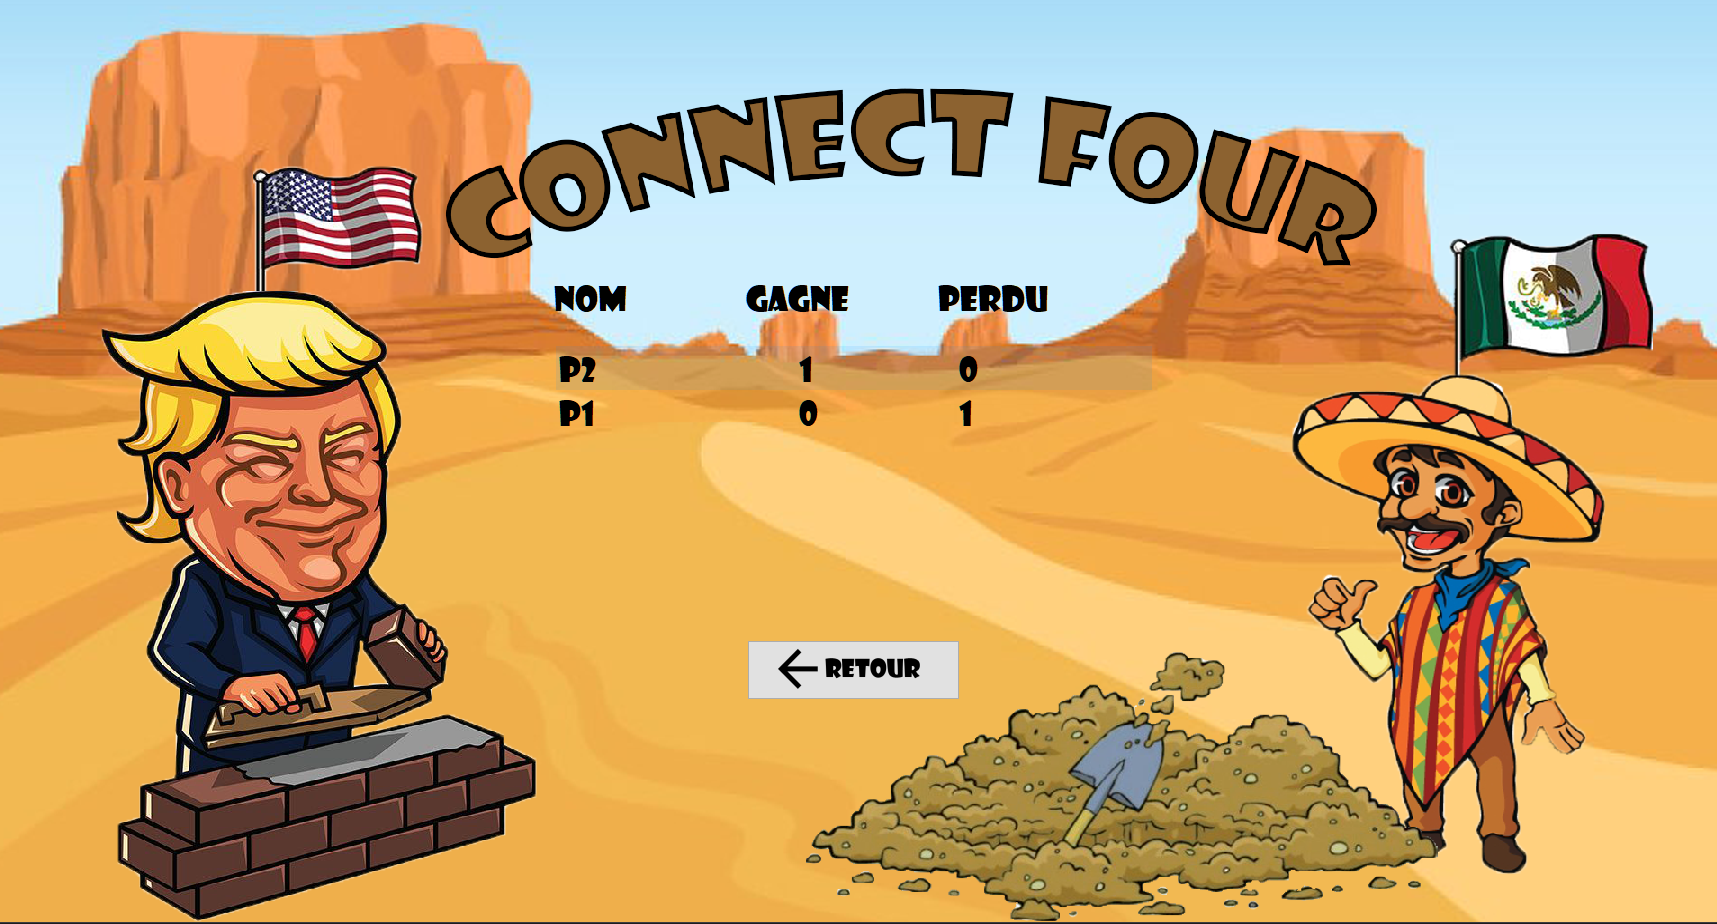
\includegraphics[width=6in]{img/4-tableauScore}
    \caption{Écran du tableau des scores}
\end{figure}

\begin{figure}[H]
    \centering
    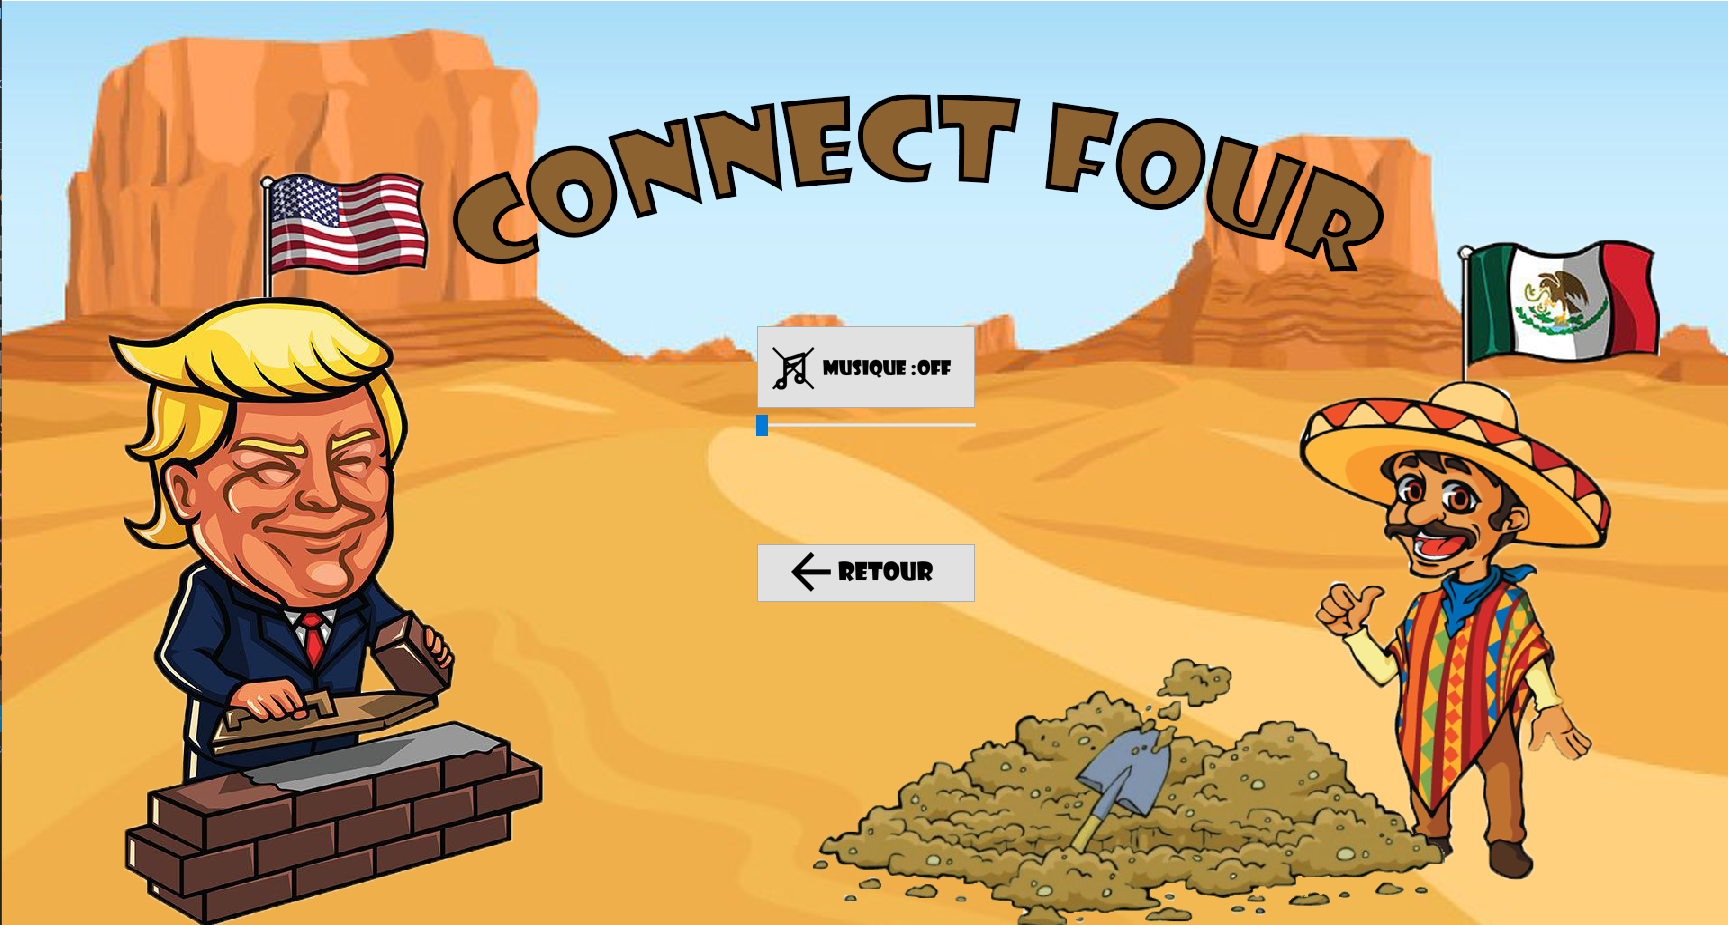
\includegraphics[width=6in]{img/5-parametres}
    \caption{Écran des paramètres généraux}
\end{figure}

\section{But, fonctionnement et guide d'usager de Conect Four}

Le but de cette application est de permettre à deux personnes de jouer au jeu puissance~4 sans l’usage de leurs mains.

De plus, la forme finale de l’application permettra de jouer contre un ordinateur à niveau de difficulté variable.
Il est possible de choisir les dimension du tableau de jeu, les noms des participants et, si l’on veut, la musique et les effets sonores.

La base de l’application est un QMainWindow ou l’on change le central widget selon ce qui est sélectionné par l’usager.
Pour le tableau de jeu, la méthode QGraphicsScene a été utilisée pour pouvoir ajouter dynamiquement des éléments à la fenêtre de jeu.

Pour jouer, il faut d'abord entrer les noms des 2 joueurs.
Le joueur no 1 sera représenté par Trump et le joueur 2 par Senor.
Pour bouger les jetons, les flèches gauche et droite sont utilisés et la barre d’espace sert à faire tomber les jetons dans le tableau.
le score global de chaque joueur sera sauvegardé automatiquement après chaque partie.

\section{Ergonomie et amélioration}

Au niveau de l'ergonomie, nous avons rempli plusieurs aspects que l'on voulait retrouver dans notre application.
Le plus important était d'avoir une boucle fonction entre les différentes fenêtres de l'application pour que l'utilisateur puisse jouer plusieurs parties à la suite sans avoir à fermer l'application.
La densité de l'affichage répond à ce que l'on cherchait à avoir donc des fenêtres pas trop surchargées et d'avoir le contenu centré.
Pour la disposition des boutons nous avons choisi de mettre les boutons de retour et de quitter à gauche ou en bas de page et les boutons jouer en haut de la page et à droite.
Ergonomiquement, cette façon de disposer les boutons est utilisée dans plusieurs applications.
Les noms et les icons des boutons sont précis pour aider à l'utilisateur de circuler de façon idéale dans l'application.

Il reste quelques améliorations à faire sur notre application pour atteindre la perfection que l'on visait.
Comme le fait de pouvoir laisser le choix au joueur de choisir qui commence à placer ses jetons.
Ensuite, il faudrait trouver une façon de faire que la fenêtre du tableau de jeu soit directement en focus pour que l'utilisateur puisse utiliser directement le clavier pour poser les jetons sans devoir clicker sur la fenêtre avant.
Suite aux tests d'intégration on a vu que notre code ne gère pas une partie égale.
Il y a donc un travail de logique à implémenter à notre application.
Pour conclure, notre application est seulement pour les joueurs, donc il n'y a rien dans l'interface qui est sur la gestion du fichier de score.
En fait, ce fichier représente une façon simplifiée d'avoir un serveur et une base de données si on veut mettre notre application en ligne.
Il faudrait donc réfléchir si on veut avoir une interface d'administration ou si la gestion de la base de données se ferait dans les logiciels de base de données.

\section{Plan de tests de Connect Four}

\begin{table}[H]
    \centering
    \caption{Plan de tests de l'interface graphique}
    \begin{tabular}{p{0.25in}p{2.5in}p{0.5in}p{2.5in}}
        \hline
        \bfseries Test & \bfseries Description et résultats & \bfseries Passé & \bfseries Justification \\
        \hline\hline
        1 & Nombre d'élément dans le menu inférieur à 7 & Oui & Tous les menus ont moins de 7 éléments \\
        2 & L'utilisateur peux revenir au menu principal en tout temps. & Non & Certains écrans ne contiennent pas bouton de retour à l'écran principal.\\
        3 & Dans le tableau de score, les scores sont aligné lorsque les noms ont 6 charactères. & Oui & Les scores sont allignés.\\
        4 & Dans le tableau de score, chaque noms n'apparait qu'une seule fois. & Non & Les nom peuvent apparaître plusieur fois.\\
        5 & La largeur de la zone de bouton est de 20\% de la largeur de la fenêtre & Oui & Les boutons ne cachent pas les images d'arrière plan.\\
        \hline
    \end{tabular}
\end{table}

\begin{table}[H]
    \centering
    \caption{Plan de tests de l'application}
    \begin{tabular}{p{0.25in}p{2.5in}p{0.5in}p{2.5in}}
        \hline
        \bfseries Test & \bfseries Description et résultats & \bfseries Passé & \bfseries Justification \\
        \hline\hline
        1 & On peux déplacer le pion de gauche à droite & Oui & Le pion se déplace de gauche à droite \\
        2 & Le pion ne peux pas aller à l'extérieur du plateu & Oui & Le déplacement du pion est limité à la largeur du plateau de jeu \\
        3 & Le jeton tombe à l'endroit attendu lorsque qu'on appuie sur la bare d'espacement & Oui & Le pion tombe au bon endroit \\
        4 & Lorsque 4 jetons sont aligné, le bon gagnant est déclaré. & Oui & Le bon gagnant est déclaré vaiceur à la fin de la partie.\\
        5 & Lorsqu'il n'est plus possible d'ajouter un jeton (le tableau est plein), l'utilisateur devrait pouvoir recommencer une autre partie.& Non & L'utilisateur reste bloqué dans le tableau.\\
        \hline
    \end{tabular}
\end{table}
